% tcm.tex

\documentclass{standalone}
\usepackage{tikz}

\usetikzlibrary{shapes, positioning, arrows.meta, decorations.pathmorphing}

\begin{document}
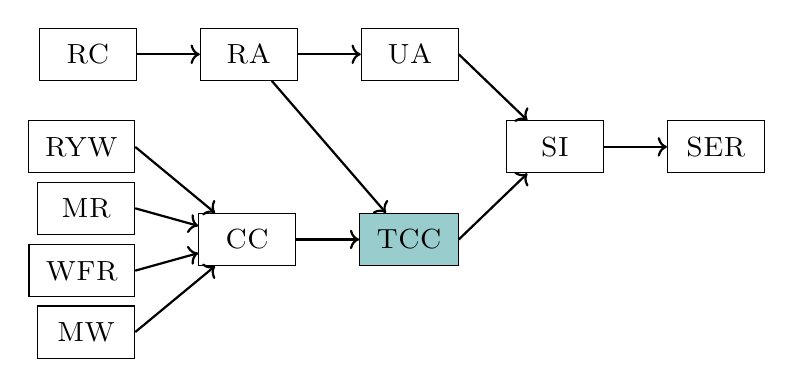
\begin{tikzpicture}[
	tcm/.style = {draw, rectangle,
	  inner sep = 6pt, minimum width = 35pt},
	every node/.append style = {anchor = center},
]
  \node[tcm] (si) {\textsc{SI}};
  \node[tcm, right = 0.80cm of si] (ser) {\textsc{SER}};

  \node[tcm, above left = 0.50cm and 0.60cm of si] (ua) {\textsc{UA}};
  \node[tcm, fill = teal!40, below left = 0.50cm and 0.60cm of si] (tcc) {\textsc{TCC}};

  \node[tcm, left = 0.80cm of ua] (ra) {\textsc{RA}};
  \node[tcm, left = 0.80cm of tcc] (cc) {\textsc{CC}};

  \node[tcm, left = 0.80cm of ra] (rc) {\textsc{RC}};

  \node[tcm, above left = 0.50cm and 0.80cm of cc] (ryw) {\textsc{RYW}};
  \node[tcm, above left = -0.28cm and 0.80cm of cc] (mr) {\textsc{MR}};
  \node[tcm, below left = -0.28cm and 0.80cm of cc] (wfr) {\textsc{WFR}};
  \node[tcm, below left = 0.50cm and 0.80cm of cc] (mw) {\textsc{MW}};

  \path[->, thick]
    (rc) edge (ra)
    (ra) edge (ua)
    (ua.east) edge (si)
    (si) edge (ser)
    (cc) edge (tcc)
    (tcc.east) edge (si)
    (ra) edge (tcc)
    (ryw.east) edge (cc)
    (mr.east) edge (cc)
    (wfr.east) edge (cc)
    (mw.east) edge (cc);
\end{tikzpicture}
\end{document}